\begin{figure}[ht!]
    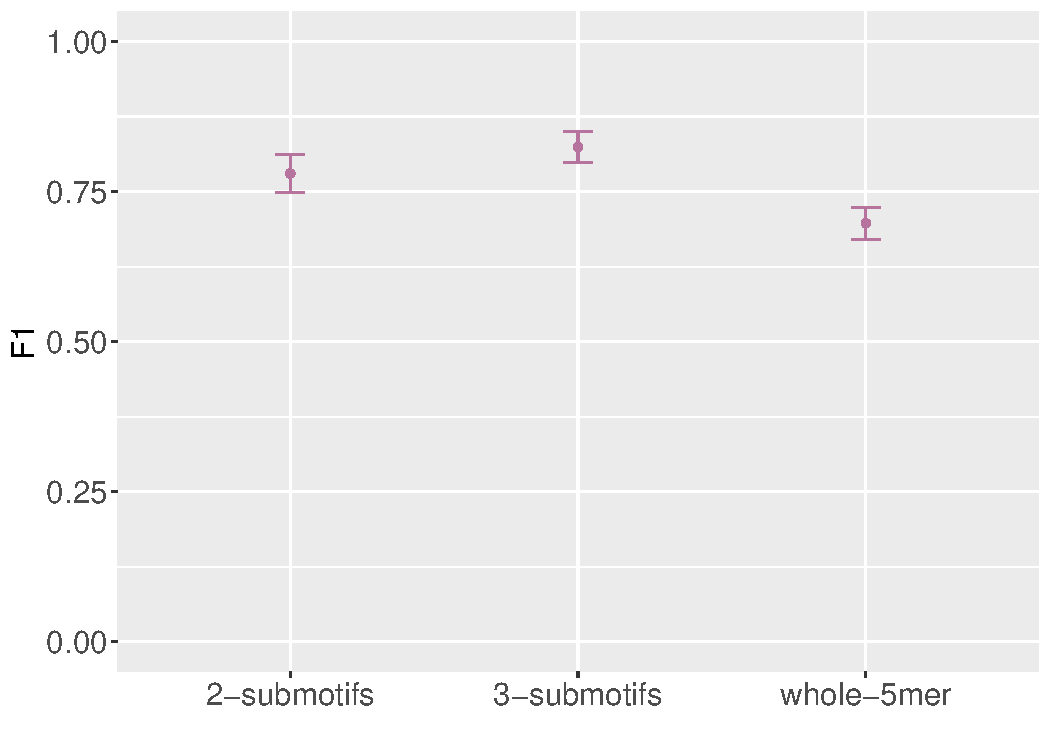
\includegraphics[scale=0.75]{graphics/f1_sce_submotif.pdf}
    \caption{\textbf{Dissecting 5-mer into multiple submotifs can potentially improve prediction accuracy compared to whole 5-mer}. Here, accuracy is shown for 5-mer when split up into 4 shorter vectors involving base substitutions and 1 flanking position (2-submotifs), 3 vectors involving base substitutions and 2 flanking positions (3-submotifs) or whole vector. For each combination of representation/metric, I iterated the training procedures of the KNN classifier 10 times using Jensen-Shannon distance. The performance of the classifier was computed based on a previously held out test data set and reported as confusion matrices and $F1$'s. The y-axis is the means of $F1$ for all representations, the error bars are the standard errors for the iterated $F1$’s. The confusion matrices are shown in Figure \ref{fig:apdx_ml_submotifs}.}
    \label{fig:f1_sce_submotif}
\end{figure}
